% Baccalauréat malgache, série C, 2008 : corrigé.
\TCDBacAttribution{C}{2008}
\providecommand{\cm}{~\mathrm{cm}}
\providecommand{\Plan}{(\mathscr{P})}
\providecommand{\dx}{~\mathrm{d}x}
\providecommand{\dt}{\mathrm{d}t}
\providecommand{\Ouv}{(O;\vec{u},\vec{v})}
\providecommand{\mes}[2]{\mathrm{mes}\left( \widehat{ \overrightarrow{#1} ; \overrightarrow{#2} } \right)}
\providecommand{\D}{(\mathscr{D})}
\providecommand{\Courbe}{(\mathscr{C})}
\providecommand{\Courben}{(\mathscr{C}_n)}
\providecommand{\CourbeU}{(\mathscr{C}_1)}
\providecommand{\CourbeD}{(\mathscr{C}_2)}
\providecommand{\bary}[1]{\mathrm{bar}\left\lbrace #1 \right\rbrace}
\providecommand{\congru}[3]{#1 \equiv #2 \quad \left[ \mathrm{mod}~#3\right]}
\providecommand{\Angl}[2]{\left( \widehat{ \overrightarrow{#1} , \overrightarrow{#2} } \right)}
%
%%%%%%%%%%%%%%%%%%%%%%%%%%%%%%%%%%%%%%%%%%%%%%%%%%%%%%%%%%%%%%%%%%%%%%%%%%%%%%%%%%%%%%%%%%%%%%%%%%%%%%%%%%%%%%%%%%%%%%%%%%%%%%%%
\noindent \underline{\textsc{\textbf{Exercice}}} (4 points)
\begin{description}
	\item[A- Probabilité]
	\begin{enumerate}
		\item Tirage simultané de trois billes : $\Comb{6}{3} = 20$ tirages équiprobables.
		\begin{itemize}
			\item \vln{Événement $E$ :}
				Avec trois billes « 12 » la somme vaut $36$ ; dès qu'une bille « 13 » est tirée la somme dépasse $36$.
				Donc $\overline{E}$ = « trois billes 12 », qui compte $\Comb{4}{3} = 4$ tirages.
				$P(E) = 1 - \frac{4}{20} = \frac{4}{5}$ : \par\noindent\ansbox{$P(E) = 0{,}80$.}
			\item \vln{Événement $F$ :}
				Il n'y a que deux billes « 13 » : trois billes de même numéro sont forcément trois billes « 12 ».
				$P(F) = \frac{4}{20}$ : \par\noindent\ansbox{$P(F) = 0{,}20$.}
		\end{itemize}
		\item \vln{Événement $G$ :}
			Tirage successif sans remise de deux billes : $6 \times 5 = 30$ résultats.
			$12^2 = 144$ et $13^2 = 169$ sont des carrés, mais $12 \times 13 = 156$ n'en est pas un ($12^2 < 156 < 13^2$).
			$G$ = « deux billes de même numéro » : $4 \times 3 + 2 \times 1 = 14$ résultats.
			$P(G) = \frac{14}{30} = \frac{7}{15}$ : \par\noindent\ansbox{$P(G) \approx 0{,}47$.}
		\item \vln{Événement $H$ :}
			Les sept tirages avec remise sont indépendants ; à chaque tirage, la probabilité de ne pas obtenir 13 est $\frac{4}{6} = \frac{2}{3}$.
			$P(H) = 1 - \left(\frac{2}{3}\right)^7 = 1 - \frac{128}{2187} = \frac{2059}{2187}$ : \par\noindent\ansbox{$P(H) \approx 0{,}94$.}
	\end{enumerate}
	\item[B- Arithmétique]
	\begin{enumerate}
		\item
		\begin{enumerate}
			\item \vln{Avec les congruences :}
				$2^6 = 64 = 5 \times 11 + 9$, donc $2^6 \equiv 9 \pmod{11}$ et $2^{6n+1} = 2 \times \left(2^6\right)^n \equiv 2 \times 9^n \pmod{11}$.
				Alors $A \equiv 9 \times 9^n + 2 \times 9^n = 11 \times 9^n \equiv 0 \pmod{11}$.
				\par\noindent\ansbox{$11$ divise $A$ pour tout $n \in \mathbb{N}$.}
			\item \vln{Par récurrence :}
				Notons $A_n = 9^{n+1} + 2^{6n+1}$. $A_0 = 9 + 2 = 11$ est divisible par $11$.
				Si $A_n = 11k$, alors
				$A_{n+1} = 9 \times 9^{n+1} + 64 \times 2^{6n+1} = 9A_n + 55 \times 2^{6n+1} = 11\left(9k + 5 \times 2^{6n+1}\right)$.
				\par\noindent\ansbox{Pour tout $n$, $A_n$ est divisible par $11$.}
		\end{enumerate}
		\item \vln{Résolution du système :}
			$3x - 2 \equiv 0 \pmod 5 \iff 3x \equiv 2 \pmod 5$. En multipliant par $2$ (inverse de $3$ modulo $5$ car $3 \times 2 = 6 \equiv 1$) :
			$x \equiv 4 \pmod 5$ ; réciproquement, si $x = 4 + 5k$, $3x - 2 = 10 + 15k$ est divisible par $5$.
			Les entiers $x = 4 + 5k$ tels que $-10 < x < 10$ correspondent à $k \in \{-2, -1, 0, 1\}$.
			\par\noindent\ansbox{$x \in \{-6 \, ; -1 \, ; 4 \, ; 9\}$.}
	\end{enumerate}
\end{description}
%%%%%%%%%%%%%%%%%%%%%%%%%%%%%%%%%%%%%%%%%%%%%%%%%%%%%%%%%%%%%%%%%%%%%%%%%%%%%%%%%%%%%%%%%%%%%%%%%%%%%%%%%%%%%%%%%%%%%%%%%%%%%%%%
\noindent \underline{\textsc{\textbf{PROBLEME I}}} (7 points) \newline
D'après la figure et la partie B (repère orthonormé $(O;\overrightarrow{OA},\overrightarrow{OB})$), le triangle $OAB$ est rectangle isocèle en $O$, de sens direct.
\begin{description}
	\item[Partie A]
	\begin{enumerate}
		\item
		\begin{enumerate}
			\item \vln{Figure :}
				Le triangle $OCB$ étant équilatéral direct, $C$ est l'image de $B$ par la rotation de centre $O$ et d'angle $-\frac{\pi}{3}$.
				\begin{center}
				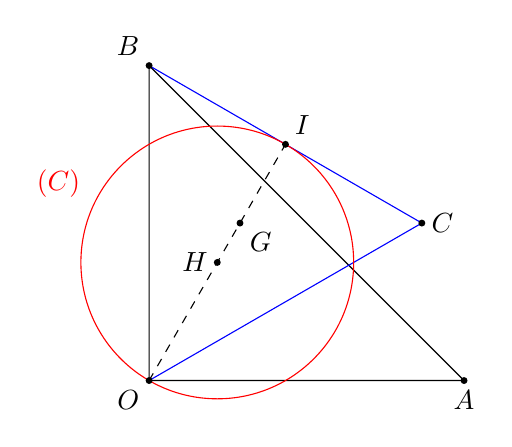
\begin{tikzpicture}[scale=.5,>=stealth]
					\coordinate (O) at (0,0); \coordinate (A) at (8,0); \coordinate (B) at (0,8);
					\coordinate (C) at (6.928,4); \coordinate (G) at (2.309,4); \coordinate (I) at (3.464,6); \coordinate (H) at (1.732,3);
					\draw (O) -- (A) -- (B) -- cycle;
					\draw[blue] (O) -- (C) -- (B);
					\draw[dashed] (O) -- (I);
					\draw[red] (H) circle (3.464);
					\foreach \P/\pos in {O/below left,A/below,B/above left,C/right,G/below right,I/above right,H/left}
						\fill (\P) circle (2.5pt) node[\pos] {$\P$};
					\node[red] at (-2.3,5) {$\Courbe$};
				\end{tikzpicture}
				\end{center}
			\item \vln{Nature de $R$ :}
				La composée de deux rotations d'angles $\frac{\pi}{3}$ et $\frac{\pi}{3}$ est un déplacement d'angle $\frac{2\pi}{3} \not\equiv 0 \pmod{2\pi}$.
				\par\noindent\ansbox{$R$ est une rotation d'angle $\frac{2\pi}{3}$.}
			\item \vln{Centre de $R$ :}
				Soit $d_1$ la bissectrice de l'angle $\widehat{COB}$ et $d_2$ la bissectrice de l'angle $\widehat{OBC}$ dans le triangle équilatéral $OCB$.
				On a $\left(d_1, (OB)\right) = \frac{\pi}{6}$ et $\left((OB), d_2\right) = \frac{\pi}{6}$ (angles de droites). Alors
				$R_O = s_{(OB)} \circ s_{d_1}$ et $R_B = s_{d_2} \circ s_{(OB)}$, d'où
				$R = s_{d_2} \circ s_{(OB)} \circ s_{(OB)} \circ s_{d_1} = s_{d_2} \circ s_{d_1}$.
				Le centre de $R$ est le point commun de $d_1$ et $d_2$ : c'est le point de concours des bissectrices du triangle équilatéral $OCB$, qui est aussi son centre de gravité.
				\par\noindent\ansbox{$R$ est la rotation de centre $G$ et d'angle $\frac{2\pi}{3}$.}
		\end{enumerate}
		\item
		\begin{enumerate}
			\item \vln{Construction de $H$ :}
				$2\overrightarrow{HO} + \overrightarrow{HB} + \overrightarrow{HC} = \vec{0}$ et $\overrightarrow{HB} + \overrightarrow{HC} = 2\overrightarrow{HI}$, donc
				$2\overrightarrow{HO} + 2\overrightarrow{HI} = \vec{0}$ : \par\noindent\ansbox{$H$ est le milieu de $[OI]$.}
			\item \vln{Ensemble $\Courbe$ :}
				Comme $H$ est le barycentre de $(O,2)$, $(B,1)$, $(C,1)$ (somme des poids $4$), la relation de Leibniz donne
				\[
					2MO^2 + MB^2 + MC^2 = 4MH^2 + 2HO^2 + HB^2 + HC^2 .
				\]
				Dans le triangle équilatéral de côté $8$, la hauteur est $OI = 4\sqrt{3}$, donc $HO = HI = 2\sqrt{3}$ et $HO^2 = 12$ ;
				$(OI) \perp (BC)$ et $IB = IC = 4$, d'où $HB^2 = HC^2 = HI^2 + IB^2 = 12 + 16 = 28$.
				La condition s'écrit $4MH^2 + 24 + 56 = 2 \times 64 = 128$, soit $MH^2 = 12$.
				\par\noindent\ansbox{$\Courbe$ est le cercle de centre $H$ et de rayon $2\sqrt{3}$ (environ $3{,}46$).}
			\item \vln{$\Courbe$ passe par $I$ :}
				$HI = \frac{OI}{2} = 2\sqrt{3}$ : \par\noindent\ansbox{$I \in \Courbe$ ;} c'est le cercle de diamètre $[OI]$ (il passe aussi par $O$), tracé sur la figure.
		\end{enumerate}
	\end{enumerate}
	\item[Partie B]
	Le repère $(O;\overrightarrow{OA},\overrightarrow{OB})$ est orthonormé car $OA = OB$ et $(OA) \perp (OB)$ ; son unité de longueur est $OA = 8\cm$.
	\begin{enumerate}
		\item \vln{Affixes :}
			$z_O = 0$, $z_A = 1$, $z_B = i$ ; $z_C = \expo{-i\frac{\pi}{3}}\, z_B = \left(\frac{1}{2} - \frac{\sqrt{3}}{2} i\right) i = \frac{\sqrt{3}}{2} + \frac{1}{2} i$ ;
			$z_G = \frac{z_O + z_B + z_C}{3} = \frac{\sqrt{3}}{6} + \frac{1}{2} i$.
			\par\noindent\ansbox{$z_O = 0$, $z_A = 1$, $z_B = i$, $z_C = \frac{\sqrt{3}}{2} + \frac{1}{2}i$, $z_G = \frac{\sqrt{3}}{6} + \frac{1}{2}i$.}
		\item
		\begin{enumerate}
			\item \vln{Angle et rapport :}
				$z_G = \frac{1}{\sqrt{3}}\left(\frac{1}{2} + \frac{\sqrt{3}}{2} i\right) = \frac{1}{\sqrt{3}}\expo{i\frac{\pi}{3}}$ :
				$OG = \frac{1}{\sqrt{3}}$ et $\Angl{OA}{OG} = \frac{\pi}{3}$.
				\par\noindent\ansbox{$\mes{OG}{OA} = -\frac{\pi}{3}$ et $\frac{OA}{OG} = \sqrt{3}$.}
			\item \vln{Éléments caractéristiques de $S$ :}
				$S(O) = O$ et $S(G) = A$ : le rapport est $\frac{OA}{OG}$ et l'angle est $\Angl{OG}{OA}$.
				\par\noindent\ansbox{$S$ : centre $O$, rapport $\sqrt{3}$, angle $-\frac{\pi}{3}$.}
			\item \vln{Expression complexe :}
				$z' = \sqrt{3}\,\expo{-i\frac{\pi}{3}} z$, soit \par\noindent\ansbox{$S : z' = \left(\frac{\sqrt{3}}{2} - \frac{3}{2} i\right) z$.}
				Vérification : $\left(\frac{\sqrt{3}}{2} - \frac{3}{2}i\right)\left(\frac{\sqrt{3}}{6} + \frac{1}{2}i\right) = \frac{1}{4} + \frac{3}{4} + i\left(\frac{\sqrt{3}}{4} - \frac{\sqrt{3}}{4}\right) = 1 = z_A$.
		\end{enumerate}
	\end{enumerate}
\end{description}
%%%%%%%%%%%%%%%%%%%%%%%%%%%%%%%%%%%%%%%%%%%%%%%%%%%%%%%%%%%%%%%%%%%%%%%%%%%%%%%%%%%%%%%%%%%%%%%%%%%%%%%%%%%%%%%%%%%%%%%%%%%%%%%%
\noindent \underline{\textsc{\textbf{PROBLEME II}}} (9 points)
\begin{description}
	\item[Partie A]
	\begin{enumerate}
		\item
		\begin{enumerate}
			\item \vln{Continuité et dérivabilité en $0$ :}
				Quand $x \to 0^+$, $-\frac{1}{nx} \to -\infty$ donc $\expo{-\frac{1}{nx}} \to 0$.
				Ainsi $\lim_{x\to 0^+} f_n(x) = 0 \times 0 = 0 = f_n(0)$ : $f_n$ est continue (à droite) en $0$.
				$\frac{f_n(x) - f_n(0)}{x - 0} = \expo{-\frac{1}{nx}} \to 0$ :
				\par\noindent\ansbox{$f_n$ est continue et dérivable en $0$, avec $f_n'(0) = 0$.}
			\item \vln{Tableau de variation :}
				Pour $x > 0$, $f_n'(x) = \expo{-\frac{1}{nx}} + x \cdot \frac{1}{nx^2}\expo{-\frac{1}{nx}} = \left(1 + \frac{1}{nx}\right)\expo{-\frac{1}{nx}} > 0$.
				En $+\infty$, $\expo{-\frac{1}{nx}} \to 1$, donc $f_n(x) \to +\infty$.
				\[
				\begin{array}{c|ccc}
					x & 0 & & +\infty \\ \hline
					f_n'(x) & 0 & + & \\ \hline
					 & & & +\infty \\
					f_n & & \nearrow & \\
					 & 0 & &
				\end{array}
				\]
		\end{enumerate}
		\item
		\begin{enumerate}
			\item \vln{Sens de variation de $g$ :}
				$g'(u) = 1 - \expo{-u} \geq 0$ pour $u \geq 0$ (car $\expo{-u} \leq 1$), nul seulement en $0$.
				\par\noindent\ansbox{$g$ est strictement croissante sur $[0;+\infty[$.}
			\item \vln{Encadrement :}
				$g(u) \geq g(0) = 0$, soit $\expo{-u} + u - 1 \geq 0$, c'est-à-dire $1 - \expo{-u} \leq u$ ; et $1 - \expo{-u} \geq 0$ car $\expo{-u} \leq 1$.
				\par\noindent\ansbox{$0 \leq 1 - \expo{-u} \leq u$ pour tout $u \geq 0$.}
			\item \vln{Deuxième encadrement :}
				L'inégalité de gauche est $g(h) \geq 0$. Pour celle de droite, posons $k(h) = \expo{-h} + h - 1 - \frac{h^2}{2}$ :
				$k'(h) = -\expo{-h} + 1 - h = (1 - \expo{-h}) - h \leq 0$ d'après (b). Donc $k$ est décroissante sur $[0;+\infty[$ et $k(h) \leq k(0) = 0$.
				\par\noindent\ansbox{$0 \leq \expo{-h} + h - 1 \leq \frac{h^2}{2}$ pour tout $h \geq 0$.}
			\item \vln{Position par rapport à $(\Delta_n)$ et asymptote :}
				Pour $x > 0$, posons $h = \frac{1}{nx} > 0$ :
				$0 \leq \expo{-\frac{1}{nx}} + \frac{1}{nx} - 1 \leq \frac{1}{2n^2x^2}$. En multipliant par $x > 0$ :
				\par\noindent\ansbox{$0 \leq f_n(x) - \left(x - \frac{1}{n}\right) \leq \frac{1}{2n^2x}$ pour tout $x > 0$.}
				Comme $\lim_{x\to+\infty} \frac{1}{2n^2x} = 0$, le théorème des gendarmes donne $\lim_{x\to+\infty}\left[f_n(x) - \left(x - \frac{1}{n}\right)\right] = 0$ :
				\par\noindent\ansbox{la droite $(\Delta_n) : y = x - \frac{1}{n}$ est asymptote à $\Courben$ en $+\infty$.}
			\item \vln{Position :}
				D'après (d), $f_n(x) - \left(x - \frac{1}{n}\right) \geq 0$ pour $x > 0$ (et même $> 0$, car $g(h) > 0$ pour $h > 0$, $g$ étant strictement croissante) ;
				en $0$ : $f_n(0) = 0 > -\frac{1}{n}$.
				\par\noindent\ansbox{$\Courben$ est au-dessus de $(\Delta_n)$ sur $[0;+\infty[$.}
		\end{enumerate}
		\item \vln{Tracé de $\CourbeD$ et $(\Delta_2)$ :}
			$f_2(x) = x\expo{-\frac{1}{2x}}$ ; $(\Delta_2) : y = x - \frac{1}{2}$. Tangente horizontale en $O$.
			Valeurs : $f_2(0{,}5) = 0{,}5\,\expo{-1} \approx 0{,}18$ ; $f_2(1) = \expo{-0{,}5} \approx 0{,}61$ ; $f_2(2) \approx 1{,}56$ ; $f_2(3) \approx 2{,}54$.
			\begin{center}
			\begin{tikzpicture}[x=2cm,y=2cm,>=stealth]
				\draw[->] (-0.5,0) -- (3.6,0) node[below] {$x$};
				\draw[->] (0,-0.7) -- (0,3.2) node[left] {$y$};
				\foreach \t in {1,2,3} \draw (\t,0.03) -- (\t,-0.03) node[below] {\small $\t$};
				\foreach \t in {1,2,3} \draw (0.03,\t) -- (-0.03,\t) node[left] {\small $\t$};
				\node[below left] at (0,0) {$O$};
				\draw[red] (0,-0.5) -- (3.5,3) node[right] {$(\Delta_2)$};
				\draw[blue,thick] (0,0) -- plot[domain=0.02:3.5,samples=120] (\x,{\x*exp(-1/(2*\x))});
				\node[blue] at (2.3,1.4) {$\CourbeD$};
			\end{tikzpicture}
			\end{center}
	\end{enumerate}
	\item[Partie B]
	\begin{description}
		\item[a)] \vln{Encadrement de $f_n(t)$ :}
			Pour $t \in ]0;1]$, $\expo{-\frac{1}{nt}} \leq 1$ donne $f_n(t) \leq t$, et A.2.(d) donne $f_n(t) \geq t - \frac{1}{n}$.
			Pour $t = 0$ : $-\frac{1}{n} \leq 0 \leq 0$.
			\par\noindent\ansbox{$t - \frac{1}{n} \leq f_n(t) \leq t$ pour tout $t \in [0;1]$.}
		\item[b)] \vln{Limite de $I_n$ :}
			En intégrant sur $[0;1]$ : $\int_0^1 \left(t - \frac{1}{n}\right)\dt \leq I_n \leq \int_0^1 t\,\dt$, soit
			$\frac{1}{2} - \frac{1}{n} \leq I_n \leq \frac{1}{2}$.
			Comme $\lim_{n\to+\infty}\left(\frac{1}{2} - \frac{1}{n}\right) = \frac{1}{2}$, par le théorème des gendarmes :
			\par\noindent\ansbox{$\lim_{n\to+\infty} I_n = \frac{1}{2}$.}
	\end{description}
	\item[Partie C]
	\begin{enumerate}
		\item \vln{Résolution de $(E')$ :}
			\ansbox{Les solutions de $y' - y = 0$ sont les fonctions $x \mapsto C\expo{x}$, $C \in \mathbb{R}$.}
		\item
		\begin{enumerate}
			\item \vln{$f$ est solution de $(E)$ :}
				Pour $x > 0$, $f'(x) = \left(1 + \frac{1}{x}\right)\expo{-\frac{1}{x}}$ (c'est $f_1'$), donc
				\[
					f'(x) - f(x) = \left(1 + \frac{1}{x} - x\right)\expo{-\frac{1}{x}} = \frac{-x^2 + x + 1}{x}\expo{-\frac{1}{x}} .
				\]
				\par\noindent\ansbox{$f$ est solution de $(E)$ sur $]0;+\infty[$.}
			\item \vln{Équivalence :}
				$(\varphi + f)' - (\varphi + f) = (\varphi' - \varphi) + (f' - f) = (\varphi' - \varphi) + \frac{-x^2+x+1}{x}\expo{-\frac{1}{x}}$.
				Donc $\varphi + f$ vérifie $(E)$ si et seulement si $\varphi' - \varphi = 0$.
				\par\noindent\ansbox{$\varphi + f$ est solution de $(E)$ $\iff$ $\varphi$ est solution de $(E')$.}
			\item \vln{Solutions de $(E)$ :}
				Toute fonction $y$ dérivable sur $]0;+\infty[$ s'écrit $y = \varphi + f$ avec $\varphi = y - f$ ; d'après (b) et 1. :
				\par\noindent\ansbox{les solutions de $(E)$ sur $]0;+\infty[$ sont $x \mapsto C\expo{x} + x\expo{-\frac{1}{x}}$, $C \in \mathbb{R}$.}
		\end{enumerate}
	\end{enumerate}
\end{description}
